\section*{Paradigme numérique}
\addcontentsline{toc}{section}{Paradigme numérique}

En général, on suppose $\eps \ll 1$, et donc le système~\eqref{sec:intro:eq:u} comporte une dynamique \textit{rapide} par rapport au temps d'étude. À cet égard, des méthodes d'\textit{analyse asymptotique} ont été développées, c'est-à-dire des méthodes qui permettent de caractériser le système dans cette limite $\eps$ \enquote{petit}, en général en découplant ces deux dynamiques. Pour les problèmes hautement oscillants, trois exemples particulièrement célèbres sont les méthodes d'homogénéisation~\cite{goudon.2003.homogenization}, de moyennisation~\cite{perko.1969.higher,sanders.2007.averaging,lochak.1988.multiphase} et de formes normales~\cite{murdock.2006.normal,bambusi.2003.birkhoff}. Pour les problèmes à relaxation rapide, la littérature est moins fournie. Qu'il s'agisse de calculer la variété centrale comme précédemment ou d'un développement de Chapman-Enskog~\cite{santos.1986.divergence,degond.2004.macroscopic,chartier.2015.uniformly}, la phase transitoire n'est pas calculée. 

Plus récemment dans \cite{castella.2016.formal}, les auteurs capturent
aussi la phase transitoire, mais la méthode n'est valide que dans la
limite $\eps \rightarrow 0$. Dans cette section, on étudie l'application
de méthodes numériques \enquote{standards} de l'état de l'art, et on
observe le comportement de l'erreur numérique non seulement en fonction
du pas de temps $\Dt$, mais aussi en fonction du paramètre $\eps$. 

On commence par décrire ce qu'on entend par \enquote{méthode numérique}
et le contexte dans lequel on va les étudier. Ensuite, on présente trois
méthodes d'ordre 2 de l'état de l'art~: le splitting de Strang, un
schéma IMEX-BDF et une méthode de Runge-Kutta exponentielle. 



\subsection*{Mise en place de la résolution}
\addcontentsline{toc}{subsection}{Mise en place de la résolution}

Pour étudier le comportement des schémas numériques sur les problèmes de la forme~\eqref{sec:intro:eq:u}, on considère l'exemple jouet suivant
\begin{subequations} \label{sec:intro:eq:jouet_v}
    \begin{empheq}[left=\left\lbrace, right=\right.]{align} &
        \pa_t v_1 = v_2 , & &
        v_1(0) = 1 , \vphantom{\frac11}\qquad\qquad
        \\ & 
        \pa_t v_2 = -\frac{1}{\eps}\big( v_1 + v_2 \big) , & &
        v_2(0) = 0 .
    \end{empheq}
\end{subequations}
Cet exemple ressemble à certains problèmes hyperboliques avec relaxation, et sa linéarité le rend simple à étudier. Il prend facilement la forme~\eqref{sec:intro:eq:xz} en posant par exemple $x = v_1$ et $z = v_1 + v_2 $, ce qui donne 
\begin{subequations} \label{sec:intro:eq:jouet_xz}
    \begin{empheq}[left=\left\lbrace, right=\right.]{align} &
        \pa_t x = -x + z , & &
        x(0) = 1 , \vphantom{\frac11}\qquad\qquad
        \\ & 
        \pa_t z = -\frac{1}{\eps}z - x + z , & &
        z(0) = 1 .
    \end{empheq}
\end{subequations}
Ce problème est linéaire et se diagonalise sans difficulté pour $\eps < 1/4$, ce qui génère
\begin{equation*}
    \newcommand{\sqEps}{\sqrt{1 - 4\eps}}
    \tilde{u} = \underbrace{\begin{pmatrix}
        -1 & 1 - r_\eps \\
        \eps & 1 - \eps - \eps r_\eps 
    \end{pmatrix}}_{\displaystyle P} \begin{pmatrix} x \\ z \end{pmatrix},
    \qquad\text{tel que}\qquad
    \pa_t \tilde{u} = \begin{pmatrix}
        -r_\eps & 0 \\ 0 & -\frac{1}{\eps} + r_\eps
    \end{pmatrix} \tilde{u}
\end{equation*}
avec $r_\eps = \frac{1}{2\eps} \big( 1 - \sqrt{1 - 4\eps} \big)$. On obtient ainsi une expression explicite pour $u = \among{x}{z}$ de la forme 
\begin{equation*}
    u(t) = P^{-1} \begin{pmatrix}
        e^{-t r_\eps} & 0 \\ 0 & e^{-t/\eps} e^{t r_\eps}
    \end{pmatrix} P u(0) 
\end{equation*}
où $P^{-1} = \frac{1}{\sqrt{1 - 4\eps}} \begin{pmatrix}
    -1 + \eps + \eps r_\eps  &  1 - r_\eps \\
                \eps         &      1
\end{pmatrix}$.
\begin{FRremark*}
    On voit bien dans la définition de $r_\eps$ que le problème change de nature entre $\eps \leq 1/4$ et $\eps > 1/4$. En effet, dans le premier cas le système est purement dissipatif, alors que dans le second, des oscillations apparaissent. Cette singularité apparaît également dans la matrice de changement de variable, dont le déterminant vaut $-\sqrt{1 - 4\eps}$.
\end{FRremark*}


En pratique, on ne sait pas résoudre tous les systèmes de la forme~\eqref{sec:intro:eq:u} de manière exacte. On va donc appliquer des méthodes d'\textit{approximation numérique} pour calculer une solution approchée. Plus spécifiquement, on va implémenter certains \textit{schémas numériques} et observer la qualité d'approximation sur l'exemple~\eqref{sec:intro:eq:jouet_xz}. Définissons ce qu'on entend par \enquote{schéma numérique}. 

On démarre par considérer une discrétisation de l'intervalle temporel $[0,T]$, c'est-à-dire qu'au lieu de considérer cet objet comme continu, on le considère comme une suite de $N+1$ points $(t_n)_{0 \leq n \leq N}$ avec $N \geq 1$. On choisit de se restreindre à une discrétisation \textit{uniforme}, c'est-à-dire que l'intervalle de temps $[0,T]$ est divisé en $N$ intervalles de taille égale notée $\Dt$. 
\begin{center}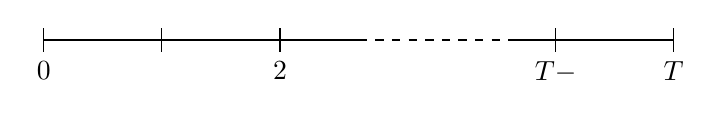
\begin{tikzpicture}
    \draw (0,0) -- (4,0);
    \foreach \x/\y in {0/$0$,1/$\Dt$,2/$2\Dt$} {
        \draw (\x*1.5,0.15cm) -- (\x*1.5,-0.15cm) node[below] {\y};
    }
    \draw[dashed] (4,0) -- (6,0);
    \draw (6,0) -- (8,0);
    \foreach \x/\y in {0/$T$,1/$T-\Dt$} {
        \draw (8-\x*1.5,0.15cm) -- (8-\x*1.5,-0.15cm) node[below] {\y};
    }
\end{tikzpicture}\end{center}
\vspace*{-12pt}
%
\noindent%
De manière équivalente, les points de séparation $(t_n)_{0 \leq n \leq N}$ sont donnés par 
\begin{equation*}
    t_{n+1} = t_n + \Dt
    \qquad\text{avec}\qquad
    t_0 = 0 \quad\text{et}\quad \Dt = \frac{T}{N} ,
\end{equation*}
ou encore $t_n = \frac{n}{N}T$. À cette discrétisation, on peut associer une \textit{approximation} $(u_n)_{0 \leq n \leq N}$ telle que $u_n \approx u(t_n)$. On peut voir un exemple d'une telle approximation en Figure~\ref{sec:intro:fig:approx_sin}, où les points carrés sont une approximation\footnote{Cette approximation est obtenue par itération en posant $\displaystyle z_{n+1} = z_n - \frac{\Dt}{\eps}z_{n+1} + \Dt \sin(t_n)$ avec $z_0 = z(0) = 1$, ce qui correspond à une méthode appelée IMEX-BDF1.} des points ronds. 

\begin{figure}[!ht]
    \centering
    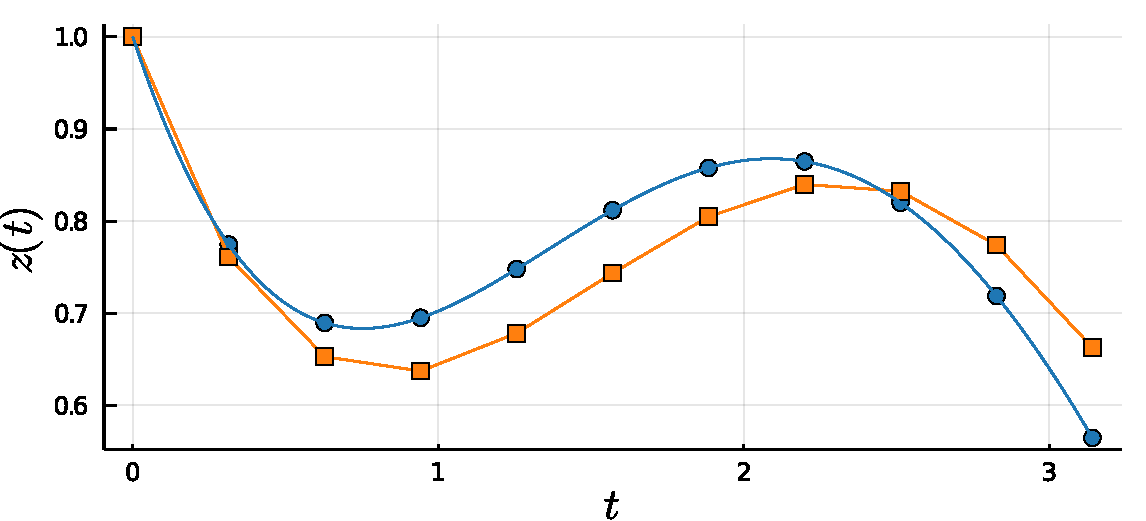
\includegraphics[width=.9\textwidth]{./Presentation/approx_sin.pdf}
    \caption{Tracé de la solution exacte (en bleu, marqueurs ronds) au problème~\eqref{sec:intro:pb:z_sin} avec $\eps = 1$ et d'une approximation (orange, marqueurs carrés) sur une discrétisation uniforme de $[0,\pi]$ à 11 points.}
    \label{sec:intro:fig:approx_sin}
\end{figure}


\begin{FRdefinition*}
    On définit l'erreur d'une approximation comme l'erreur maximale sur les points d'interpolation, i.e. étant donnée une discrétisation à $N+1$ points $(t_n)_{0 \leq n \leq N}$ et une approximation $(u_n)$ d'une fonction $t \mapsto u(t)$, l'erreur est définie par la formule 
    \begin{equation} \label{sec:intro:def:err}
        \err = \max_{0 \leq n \leq N}\big| u_n - u(t_n) \big| .
    \end{equation}
    Si en outre la solution et l'approximation dépendent du paramètre~$\eps \in (0,\eps_0]$, on écrit $\err(\eps)$ l'erreur d'approximation, et on définit l'erreur uniforme $\overline{\err}$ par 
    \begin{equation}
        \overline{\err} = \sup_{\eps \in (0,\eps_0]} \err(\eps) .
    \end{equation}
    Ces deux erreurs peuvent avoir des comportements différents.
\end{FRdefinition*}
Parfois, l'erreur est définie comme l'erreur au temps final, ce qui peut paraître moins contraignant mais a peu d'influence en pratique car les estimations d'erreur sont croissantes avec l'indice~$n$. Ainsi ces deux définitions coïncident pour les résultats théoriques.

\begin{FRremark*}
    À partir d'une approximation $(u_n)$, on peut obtenir une approximation sur une discrétisation plus fine par interpolation (typiquement avec des splines cubiques ou de manière linéaire comme en Figure~\ref{sec:intro:fig:approx_sin}). Il semble alors naturel de se demander s'il est possible de réduire le coût de calcul en calculant une approximation sur une discrétisation grossière pour l'interpoler ensuite vers une discrétisation plus fine. Néanmoins, si l'erreur telle que définie en~\eqref{sec:intro:def:err} est mauvaise, on ne peut pas espérer l'améliorer par interpolation. C'est pourquoi ce manuscrit se concentre sur cette approche \enquote{simple} de l'erreur.
\end{FRremark*}

Lorsqu'il s'agit de trouver une approximation à une solution d'équation différentielle, il semble naturel de procéder de manière itérative: les seules données accessibles sont la condition initiale $u(0)$ et le champ de vecteurs suivi par la solution, donc il faut trouver un moyen de combiner ces deux informations pour obtenir une approximation $u_1 \approx u(\Dt)$. Une fois cette information obtenue, on peut l'utiliser avec les autres pour calculer $u_2 \approx u(2\Dt)$, etc. Dans les faits, on se limite à un nombre fixe $s \geq 1$ de points pour extrapoler le suivant. On parle alors de méthode multipoints. Les méthodes à un point sont appelées méthodes de Runge-Kutta.

La méthode utilisée pour calculer un terme à partir des précédents est appelé un schéma numérique~$\Phi^\eps_{\Dt}$, et elle peut s'écrire 
\begin{equation*}
    u_{n+s} = u_{n+s-1} + \Dt\, \Phi^{\eps}_{\Dt} (u_{n+s-1}, \ldots, u_n) .
\end{equation*}
Cette notation peut être pratique pour étudier le schéma, mais il faut garder à l'esprit qu'elle peut camoufler de nombreuses difficultés. Par exemple, le schéma d'Euler implicite s'écrit 
\begin{equation*}
    u_{n+1} = u_n + \Dt \left( 
        - \frac{1}{\eps}A u_{n+1} + f(u_{n+1}) 
    \right) .
\end{equation*}
Pour trouver $\Phi^\eps_{\Dt}$, il faut inverser cette relation; on parle de schéma \textit{implicite}, par opposition aux schémas \textit{explicites}. Cette inversion peut s'avérer particulièrement coûteuse si $f$ présente des non-linéarités et si le système est grand. Ainsi par la suite on se limite à des schémas \textit{explicites} en $f$, et on fait l'hypothèse suivante~:
\begin{FRassumption*}
    On sait calculer $t \mapsto e^{-tA}$ et $t \mapsto (\id + t A)^{-1}$ de manière exacte. 
\end{FRassumption*}
\noindent%
Calculer le semi-groupe $t \mapsto e^{-tA}$ peut sembler contraignant, mais rappelons nous qu'on se restreint ici au cas où $A$ est une matrice diagonale. 


\begin{FRdefinition*}
    On dit qu'un schéma numérique~$\Phi_{\Dt}$ est d'ordre $q$ s'il existe une constante $C > 0$ et un pas de temps maximal $\Dt_0 > 0$ tel que pour toute subdivision de pas de temps $\Dt \leq \Dt_0$, l'erreur de schéma est bornée par $C\Dt^q$. 
\end{FRdefinition*}
%
\noindent%
Dans le contexte d'un schéma qui dépend du paramètre~$\eps$, la constante d'erreur $C$ et le pas de temps maximal $\Dt_0$ dépendent généralement de $\eps$, ainsi il faut distinguer l'ordre du schéma (calculé pour $\Dt \ll \eps$) de l'ordre de \enquote{convergence uniforme} du schéma, qui fait disparaître la dépendance en~$\eps$. Cette distinction sera clarifiée par les exemples à venir.



\subsection*{Méthodes numériques}
\addcontentsline{toc}{subsection}{Méthodes numériques}

On présente les résultats associés à trois méthodes d'ordre 2, qui traitent la partie raide différemment de la partie non-raide. Les méthodes sont bien définies  dans la limite $\eps \rightarrow 0$, et on s'intéresse au comportement de l’erreur en fonction de $\Dt$ \textit{et} de $\eps$.

On ne considèrera pas de méthodes complètement implicites parce qu'elles sont très coûteuses notamment dans un contexte d'EDP. Néanmoins la convergence de ces méthodes est souvent excellente et des implémentations très efficaces existent. La référence sur le sujet est~\cite{hairer.1996.solving}, et toutes les bonnes boîtes à outils de résolution d'EDO contiennent la méthode RadauII.\footnote{Attention cependant, la plupart de ces boîtes à outils masquent la difficulté associée aux méthodes implicites, à savoir la résolution d'un système et l'erreur associée. En outre, il est parfois difficile de désactiver le pas de temps adaptatif, ce qui est problématique pour une étude de convergence.} On ne considère pas non plus de méthodes purement explicites demandant $\Dt < \eps$, ce qui est beaucoup trop coûteux en pratique. 

Il est important de noter que cette introduction ne présente pas une étude des schémas présentés. Il s'agit d'une compilation non-exhaustive de résultats et d'observations sur les propriétés de ces méthodes appliquées à~\eqref{sec:intro:eq:u} afin de contextualiser les contributions du manuscrit par la suite. Néanmoins, les schémas sont présentés plus en détails dans l'Annexe~\ref{chap:schemas}.



\paragraph{Splitting de Strang\\}

Une approche courante consiste à séparer le problème~\eqref{sec:intro:eq:u} en deux parties, l'une raide et l'autre non-raide. La manière naturelle de procéder fournit
%
\begin{empheq}[left=\left\lbrace, right=\right.]{align*} &
    \pa_t u^{(1)} = -\frac{1}{\eps}A u^{(1)} ,
    \\ &
    \pa_t u^{(2)} = f(u^{(2)}) . \vphantom{\frac11}
\end{empheq}
%
On note $\varphi_t$, $\varphi^{(1)}_t$ et $\varphi^{(2)}_t$ les $t$-flots associés aux problèmes en $u$, $u^{(1)}$ et $u^{(2)}$ espectivement. On remarque qu'il est simple de calculer $\varphi^{(1)}$ de manière exacte, et simple de calculer $\varphi^{(2)}$ de manière numérique. Cependant, ces deux dynamiques sont mélangées dans $\varphi$, ce qui rend le flot du problème d'origine difficile à calculer. Ainsi, on est en droit de se poser la question~: est-il possible d'obtenir $\varphi$ à partir de $\varphi^{(1)}$ et de $\varphi^{(2)}$~? 

La réponse est négative en général, mais on peut \textit{approcher} $\varphi$ à partir de~$\varphi^{(1)}$ et de~$\varphi^{(2)}$ à l'aide de compositions successives. C'est cette approche qu'on appelle \textit{splitting}. Le plus couramment utilisé est le splitting de Strang, qui s'écrit 
\begin{equation*}
    \varphi_t = \varphi^{(1)}_{t/2} \circ \varphi^{(2)}_{t} \circ \varphi^{(1)}_{t/2} + \bigO(t^3) 
\end{equation*}
avec la constante d'erreur dans $\bigO(t^3)$ qui dépend du paramètre~$\eps$ de manière raide. Pour la plupart des équations, l'ordre des opérations n'a pas d'importance, mais lorsque le système présente une partie de relaxation raide comme ici, il a été remarqué dans~\cite{sportisse.2000.analysis,descombes.2004.operator} qu'il vaut mieux \enquote{terminer} par la relaxation. 

Notons que le splitting de Strang peut être obtenu par \enquote{symétrisation} du splitting de Lie $\varphi^{(2)}_{t} \circ \varphi^{(1)}_{t}$, d'ordre 1. 
% Attention, $\Phi_t$ n'est pas un $t$-flot au même sens que $\varphi_t$, c'est la solution particulière d'une EDO dans l'espace des morphismes. Dans le cas où $f$ est linéaire, on dispose de la formule de Baker-Campbell-Hausdorff (BCH),\todo{REF BCH}
% \begin{equation*}
%     \log \big( \Phi_t \big)
%     = t\left(\frac{-1}{\eps}A + f\right) 
%     - \frac{t^2}{2\eps} \left[A, f\right]
%     + \frac{t^3}{12\eps^2}\big( [A,[A,f]] + \eps [f,[A,f]] \big)
%     + \ldots
% \end{equation*}
% avec $[f,g] = fg - gf$ le commutateur de champs linéaires. Cette formule n'est valide que formellement, c'est-à-dire qu'elle ne converge pas forcément et que l'important est le terme général qui la génère. On peut la comparer à un développement de Taylor qu'on a poussé à un ordre \enquote{infini}. L'objet obtenu est une série entière en $t$, mais celle-ci peut avoir un rayon de convergence nul. Néanmoins, les termes de la série ont du sens et on peut en prendre les premiers termes pour construire des approximations, bien qu'il faille être prudent avec la régularité de la fonction pour obtenir des résultats rigoureux.
Le splitting est exact si et seulement si les champs $A$ et $f$ commutent, c'est-à-dire si on vérifie l'identité 
\begin{equation*}
    Af - \pa_u f \cdot A = [A,f] = 0 .
\end{equation*}
Dans ce cas, le splitting de Lie génère un flot qui coïncide avec $\varphi$. Évidemment, ce n'est pas le cas en général. En particulier dans le cas test~\eqref{sec:intro:eq:jouet_xz}, on a $[A,f] = \begin{pmatrix} 0 & -1 \\ -1 & 0 \end{pmatrix}$, donc on s'attend à avoir une erreur qui décroit comme $\Dt^2$ lors de la simulation. Cependant, on observe un résultat différent en Figure~\ref{sec:intro:fig:strang}.


% \begin{itemize}
%     \item Le morphisme $\Phi_t$ est un flot;
%     \item $\Phi_t$ et $\varphi_t$ coincïdent en tout $t$;
%     \item Les champs $A$ et $f$ commutent.
% \end{itemize}
% Le morphisme $\Phi_t$ est un flot si et seulement si cette expression est linéaire en $t$, or ce n'est pas le cas en général. Le seul moyen que ce soit le cas est que $A$ et $f$ commutent. Ce résultat est aussi valide dans le cas non-linéaire, avec le commutateur
% \begin{equation*}
%     [f,g] = \pa_u f \cdot g - \pa_u g \cdot f 
% \end{equation*}
% qui définit une algèbre de Lie sur les champs de vecteurs. Ceci correspond à une manière plus géométrique de considérer les champs de vecteurs qui revient à les associer à l'opérateur de transport $\mathcal{D}_f(g) = \pa_u g \cdot f$. Ainsi, $[f,g] = \mathcal{D}_g(f) - \mathcal{D}_f(g)$. 

% On définit l'erreur de splitting 
% \begin{equation*}
%     \err_{\mathrm{Lie}} 
%     = \log \big( \Phi_t \big) - t\left(\frac{-1}{\eps}A + f\right) 
% \end{equation*}
% qui permet d'obtenir l'erreur de troncature du schéma par un passage à l'exponentielle. Il apparaît à partir de la formule de BCH que cette erreur est de taille $t^2/\eps$, pas indépendante de $\eps$. Néanmoins, on a déjà vu avec Euler implicite que l'accumulation d'erreur pouvait devenir indépendante de $\eps$, grâce aux propriétés de décroissance de $z$. C'est le cas ici, et on peut borner l'erreur \textit{indépendamment} de $\eps$. 

% On cherche ensuite à améliorer la convergence du schéma: il serait agréable de pouvoir profiter d'une convergence à un ordre plus élevé. La méthode généralement considérée est le splitting de Strang~:
% \begin{equation*}
%     \varphi_t \approx \varphi^{(1)}_{t/2} \circ \varphi^{(2)}_{t} \circ \varphi^{(1)}_{t/2} .
% \end{equation*}
% Cette méthode a l'avantage d'être d'ordre 2, et de présenter des propriétés géométriques sympathiques de par sa symétrie (elle génère d'ailleurs la méthode de Störmer-Verlett, voir Annexe~\textbf{REF}\todo{Storm-Verl}). Néanmoins, il n'est pas clair qu'elle présente un bon comportement lorsque la raideur augmente, i.e. lorsque $\eps$ diminue. En effet, un calcul de l'erreur de troncature donne 
% \begin{equation*}
%     \varphi_t - \varphi^{(1)}_{t/2} \circ \varphi^{(2)}_{t} \circ \varphi^{(1)}_{t/2} 
%     = \frac{t^3}{12\eps^2} \big( [A,[A,f]] + \eps [[A,f],f] \big)
%     + \bigO(t^4) .
% \end{equation*}
% Ainsi, même si un $1/\eps$ est compensé par la décroissance rapide de $z$, l'erreur ne sera pas indépendante de $\eps$. On peut vérifier ce résultat de manière numérique.


\begin{figure}
    \centering
    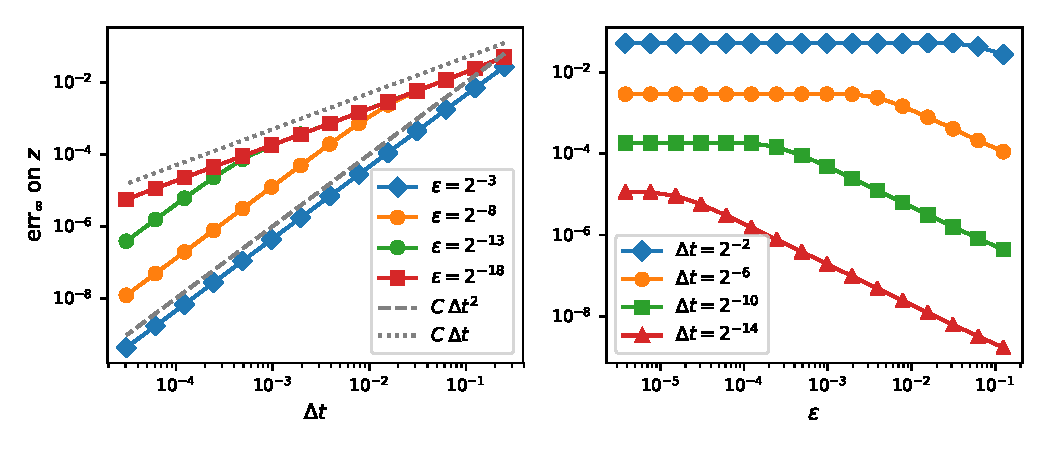
\includegraphics[width=\textwidth]{./Presentation/strang_err_x.pdf}
    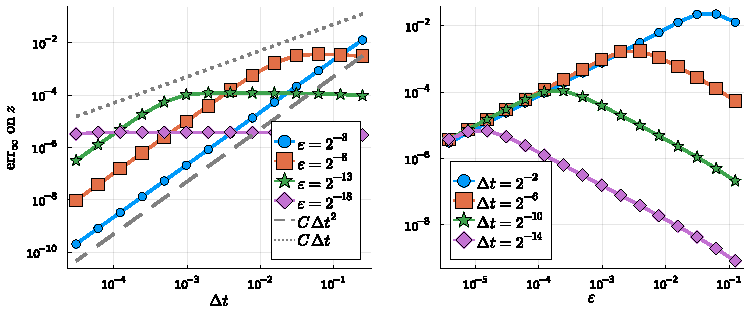
\includegraphics[width=\textwidth]{./Presentation/strang_err_z.pdf}
    \caption{Erreurs sur $x$ (en haut) et $z$ (en bas) en fonction de $\Dt$ (à gauche) et de $\eps$ (à droite) avec la méthode de Strang. Sur les tracés de l'erreur en fonction de $\Dt$, les convergences théorique et uniforme sont tracées.}
    \label{sec:intro:fig:strang}
\end{figure}

Dans cette figure, on observe que le comportement de la solution est celui attendu pour $\Dt \ll \eps$. Néanmoins, lorsqu'on trace l'erreur en fonction de $\eps$, on voit qu'à $\Dt$ fixé, il y a toujours un seuil à partir duquel une réduction de $\eps$ entraîne une augmentation de l'erreur. Cette augmentation entraîne une \textit{réduction d'ordre}, c'est-à-dire qu'on ne peut pas avoir
\begin{equation*}
    \sup_{0 < \eps \leq \eps_0} \err \leq C \Dt^q ,
\end{equation*}
avec $q = 2$, ce n'est possible qu'avec $q = 1$. Cette réduction d'ordre a été notée dans différents contextes \cite{sportisse.2000.analysis,faou.2015.analysis}, et différentes méthodes ont été développées pour dépasser cette limite \cite{einkemmer.2015.overcoming,cano.2017.avoiding,bertoli.2020.strang}, même si la méthode reste au plus d'ordre~2.

% \todo[inline]{Expliquer un peu mieux les graphes}
% \todo[inline]{Faire une colormap d'erreur avec $\Dt$ et $\eps$ en coordonnées pour mieux discuter du comportement asymptotique $\eps \rightarrow 0$ du schéma.}


\paragraph{Méthodes exponentielles Runge-Kutta (expRK)\\}

Ces méthodes exponentielles\footnote{À ne pas confondre avec les méthodes de Lawson (voir~\cite{lawson.1967.generalized,hochbruck.2020.convergence}) qui procèdent en applicant des méthodes de Runge-Kutta standards sur la variable filtrée $v(t) = e^{t A/\eps}u(t)$, puis en multipliant le résultat par $e^{-t A/\eps}$. Les résultats théoriques sur la convergence de ces dernières sont encore très récents.} proviennent de la formulation intégrale du problème~\eqref{sec:intro:eq:u}, 
\begin{equation*}
    u(t) = e^{-\frac{t}{\eps}A}u_0 + \int_0^t e^{-\frac{t-\tau}{\eps}A} f(u(s)) \D s .
\end{equation*}
La partie du semi-groupe est gardée exacte tandis que la partie (possiblement) non-linéaire est approchée, ce qui conduit au schéma d'ordre 1 suivant,
\begin{equation} \label{sec:intro:eq:expEuler}
    u_{n+1} = e^{-\Dt A/\eps} u_n + \left(\int_0^{\Dt} e^{(\tau-\Dt) A/\eps} \D\tau \right) f(u_n) .
\end{equation}
Pour passer à l'ordre supérieur, les parties raide et non-raide sont liées, donc l'approche demande plus de subtilité, mais on peut obtenir des méthodes exponentielles Runge-Kutta (i.e. des méthodes à un pas, pour obtenir $u_{n+1} \approx u(t_{n+1})$ à partir de seulement $u_n \approx u(t_n)$) d'ordre arbitraire. Une grande classe de schémas de ce type est compilée dans~\cite{hochbruck.2005.explicit}, et dans un autre article les mêmes auteurs obtiennent une convergence théorique. 

\medskip\noindent%
\textit{Erreur de convergence} (Hochbruck, Ostermann - \cite{hochbruck.2004.exponential})

Avec un schéma expRK d'ordre~$q \geq 1$, l'erreur vérifie la borne à une constante multiplicative près
\begin{equation*}
    \left| 
        \left( I + \frac{1}{\eps}A \right) \big( u_n - u(t_n) \big) 
    \right|
    \leq \Dt^{q} \left( 
        \sup_{0 \leq t \leq t_n} \big| \pa_t^{\: q-1} \mathcal{U}(t) \big| 
        + \int_0^{t_n} \big| \pa_t^{\: q} \mathcal{U}(t) \big| \D t 
    \right) 
\end{equation*}
où $\mathcal{U} = \pa_t u + \frac{1}{\eps}Au$. 

\medskip%
Ce résultat est généralement évoqué dans un contexte fonctionnel de problème parabolique, mais cette version simplifiée est suffisante ici. Un intérêt remarquble de ces méthodes est que dans l'erreur, la composante~$z$ est renormalisée par~$\eps$. Dans notre cas, cela permet d'obtenir une sorte d'erreur relative puisque $z(t) = \eps h^\eps(x(t)) + \bigO(e^{-t/\eps})$. D'ailleurs, le schéma~\eqref{sec:intro:eq:expEuler} (parfois appelé \enquote{Euler exponentiel}) avait été proposé dans~\cite{verwer.1998.note} pour obtenir une meilleure convergence que le splitting de Strang en erreur relative. 

\begin{figure}[!h]
    \centering
    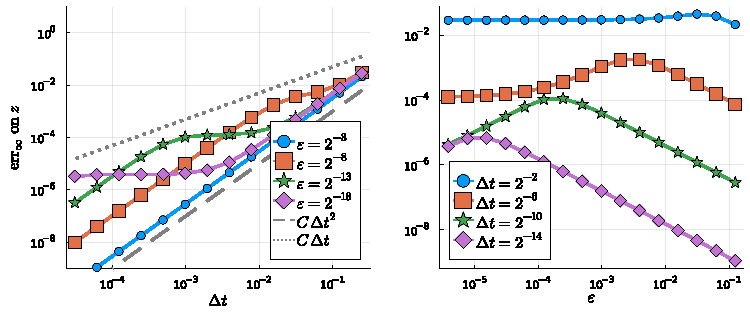
\includegraphics[width=\textwidth]{./Presentation/rk2_err_x.pdf}
    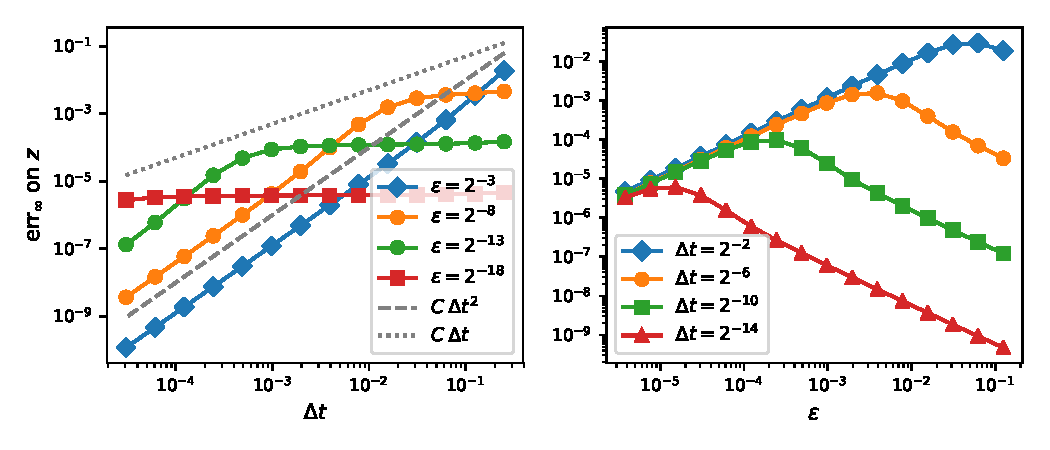
\includegraphics[width=\textwidth]{./Presentation/rk2_err_z.pdf}
    \caption{Erreurs sur $x$ (en haut) et $z$ (en bas) en fonction de $\Dt$ (à gauche) et de $\eps$ (à droite) avec le schéma exponentiel RK2. Sur les tracés de l'erreur en fonction de $\Dt$, les convergences théorique et uniforme sont tracées.}
    \label{sec:intro:fig:rk2}
\end{figure}

Cette renormalisation par~$\eps$ de la composante~$z$ se voit nettement en Figure~\ref{sec:intro:fig:rk2} sur l'erreur en fonction de~$\eps$ est bornée par une fonction de la forme~$C\eps$. Sur~$x$, à $\eps$ fixé, on observe trois phases dans les variations d'erreur en fonction de $\Dt$:
\begin{itemize}
    \item une décroissance en $\Dt^2$;
    \item un plateau à partir de $\Dt^2 \approx \eps$ jusqu'à $\Dt \approx \eps$;
    \item de nouveau une décroissance en $\Dt^2$.
\end{itemize}
Cette deuxième phase engendre une réduction d'ordre, où l'ordre \enquote{uniforme} est 1, et la troisième phase présente l'ordre \enquote{naturel} du schéma. Pour la composante~$z$, il n'y a pas de première phase, mais la réduction d'ordre est la même. Malgré cela, la convergence est meilleure que pour le splitting de Strang~: dans le paradigme $\eps \rightarrow 0$, seule la première phase est observée et l'erreur décroit comme $\Dt^2$. On dit que le schéma \enquote{préserve l'asymptote}. Cette description ne permet pas de décrire le comportement de l'erreur dans les phases 1 et 3, mais pas dans la phase 2. 

% \todo[inline]{Faire une colormap d'erreur avec $\Dt$ et $\eps$ en coordonnées pour mieux discuter du comportement asymptotique $\eps \rightarrow 0$ du schéma. Notamment, si on pose $\eps = 0$ la convergence est d'ordre 2.}



\paragraph{Méthode IMEX-BDF\\}


L'inconvénient des méthodes exponentielles est qu'elles demandent une intégration très précise du semi-groupe $t \mapsto e^{-tA/\eps}$. On peut considérer des méthodes moins coûteuses, qui demandent seulement d'inverser un système linéaire. C'est le cas par exemple des méthodes implicite-explicites (IMEX), où la partie raide est implicite et la partie non-linéaire est explicite. Ainsi la méthode d'Euler implicite-explicite appliquée à~\eqref{sec:intro:eq:u} s'écrit
\begin{equation*}
    \frac{u_{n+1} - u_n}{\Dt} = -\frac{1}{\eps}A u_{n+1} + f(u_n) .
\end{equation*}
On se restreint ici aux méthodes multipas dénommées IMEX-BDF (\textit{backwards differentiation formula}), initialement développées dans~\cite{crouzeix.1980.methode}, puis dans~\cite{ascher.1995.implicit,akrivis.1999.implicit,hundsdorfer.2007.imex,dimarco.2017.implicit}. On a là aussi une erreur théorique.

\bigskip\noindent%
\textit{Résultat sur l'erreur} (Crouzeix - \cite{crouzeix.1980.methode})

Avec une méthode IMEX-BDF d'ordre~$q$ à~$s$ pas, si on suppose qu'on a pu obtenir les $(s-1)$-ièmes premiers pas avec une manière quelconque, l'erreur sur les pas suivants peut être bornée par 
\begin{equation*}
    \big| u_n - u(t_n) \big| \leq
    \sum_{i = 0}^{s-1} \big| u_i - u(t_i) \big|
    + \Dt^q \int_0^{t_n} \left( 
        \big| \pa_t^{\: q+1} u(t) \big| 
        + \frac{1}{\eps} \big| A \pa_t^{\: q} u(t) \big| 
    \right) \D t 
\end{equation*}
à une constante multiplicative près.

\medskip
La différence principale de cette erreur avec celle des méthodes expRK est que la composante~$z$ n'est pas \enquote{normalisée}. On voit ainsi en Figure~\ref{sec:intro:fig:bdf2} que l'erreur uniforme sur $z$ dégénère à l'ordre \textit{zéro}. Il est même possible d'augmenter l'erreur en diminuant le pas de temps~$\Dt$. 

\begin{figure}[!h]
    \centering
    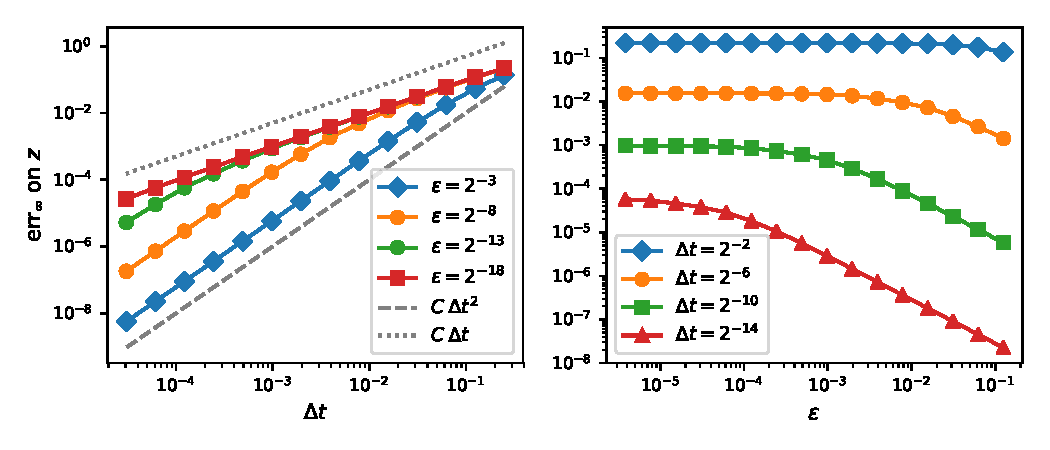
\includegraphics[width=\textwidth]{./Presentation/bdf2_err_x.pdf}
    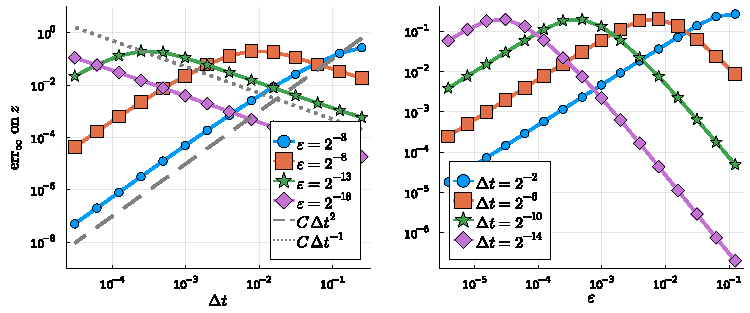
\includegraphics[width=\textwidth]{./Presentation/bdf2_err_z.pdf}
    \caption{Erreurs sur $x$ (en haut) et $z$ (en bas) en fonction de $\Dt$ (à gauche) et de $\eps$ (à droite) avec le schéma IMEX-BDF2. Sur les tracés de l'erreur en fonction de $\Dt$, la convergence théorique est tracée, ainsi que pour $x$ la convergence uniforme et pour $z$ l'ordre négatif observé sur une portion de valeurs de $\Dt$.}
    \label{sec:intro:fig:bdf2}
\end{figure}

Ces méthodes sont néanmoins très utilisées, notamment dans le contexte de modèles cinétiques. Par exemple les méthodes IMEX-LM développées dans~\cite{lemou.2008.new,boscarino.2017.unified,albi.2020.implicit} sur un système 
\begin{equation*}
    \pa_t \rho + \pa_x j = 0, \qquad 
    \pa_t j + \frac{1}{\eps} \pa_x \rho = -\frac{1}{\eps}j 
\end{equation*}
traitent de manière la partie en~$j$ en gardant explicite la partie en~$\rho$. Cela permet d'avoir des schémas qui se comportent bien dans la limite $\eps \rightarrow 0$ malgré la raideur sur le transport en~$\rho$. 

En outre, si la donnée initiale se situe proche de l'équilibre $z = \eps h^\eps(x)$ de sorte que $\pa_t^{\: q+1} u$ reste bornée dans la limite~$\eps \rightarrow 0$, alors on peut obtenir une convergence uniforme. On peut voir une interprétation de ce résultat en Figure~\ref{sec:intro:fig:bdf2_z0} où l'erreur sur~$z$ est améliorée en prenant une donnée initiale nulle.\footnote{Le même phénomène est observé pour le schéma expRK.} Ainsi, il est fréquent de choisir une donnée initiale bien préparée et d'annoncer que ce type de schéma est \enquote{uniformément précis}, par exemple dans~\cite{jin.2000.uniformly,hu.2021.uniform}. La même confusion est faite pour les schémas IMEX-RK dans~\cite{boscarino.2009.class,boscarino.2017.unified}, par exemple. 

\begin{figure}[!h]
    \centering
    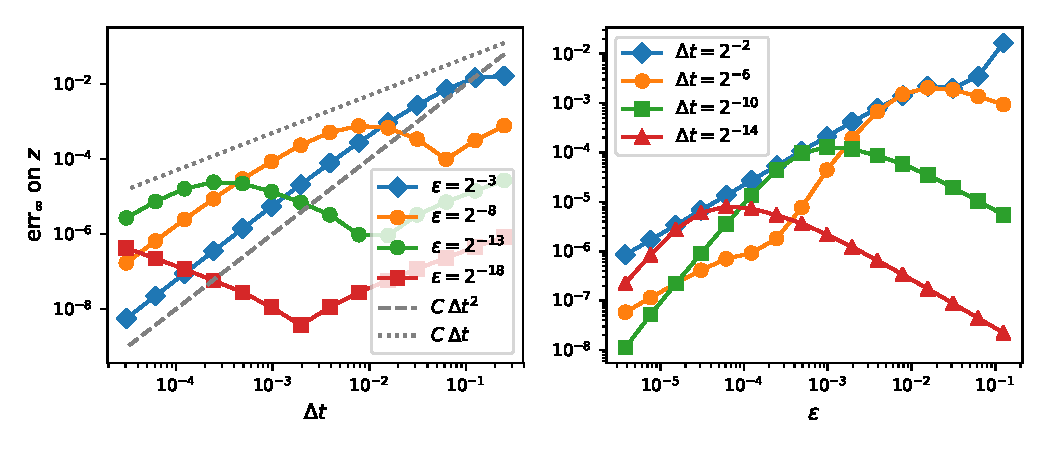
\includegraphics[width=\textwidth]{./Presentation/bdf2_err_z0.pdf}
    \caption{Erreur sur $z$ en fonction de $\Dt$ (à gauche) et de $\eps$ (à droite) avec le schéma IMEX-BDF2, avec une donnée initiale~$z(0) = 0$. Sur les tracés de l'erreur en fonction de $\Dt$, les convergences théorique et uniforme sont tracées.}
    \label{sec:intro:fig:bdf2_z0}
\end{figure}



\subsection*{D'autres notions de convergence}
\addcontentsline{toc}{subsection}{D'autres notions de convergence}

On voit que toutes ces méthodes subissent une réduction d'ordre: on passe d'une convergence d'ordre~2 à une convergence d'ordre~1, ou pire. Pourtant, les schémas sont bien \textit{d'ordre~2} au sens asymptotique $\Dt \rightarrow 0$, comme on l'observe pour $\eps = 2^{-3}$ en Figures~\ref{sec:intro:fig:strang}, \ref{sec:intro:fig:rk2} et~\ref{sec:intro:fig:bdf2}. Il apparaît donc nécessaire d'introduire des concepts de convergence qui diffèrent des définitions usuelles. 

\begin{FRdefinition*}
    Considérons la solution $t \mapsto u^\eps(t)$ du problème~\eqref{sec:intro:eq:u} avec une donnée initiale~$u(0) = u_0$ indépendante de~$\eps$. On construit une solution approchée~$(u^\eps _n)$ en appliquant un schéma~$\Phi^\eps _{\Dt}$ d'ordre $q \geq 1$, et on suppose que $\Phi^\eps_{\Dt}$ admet une limite $\eps \rightarrow 0$, qu'on note~$\Phi^0_{\Dt}$. 

    On dit que le schéma~$\Phi_{\Dt}^\eps$ est \emph{asymptotic preserving} (AP) ou qu'il préserve l'asymptote si le schéma limite~$\Phi^0_{\Dt}$ existe et est du même ordre $q$ que le schéma d'origine. On dit en outre que le schéma est \emph{uniformly accurate} (UA) ou uniformément précis si l'erreur uniforme présente le même ordre de convergence que l'erreur \enquote{standard} du schéma. 
\end{FRdefinition*}

On peut résumer ces propriétés sur le diagramme de commutation suivant~:
\begin{center}
    \begin{tikzpicture}[baseline= (a).base]
        \node[scale=1.3] (a) at (0,0){
\begin{tikzcd}[row sep=huge, column sep=huge]
    u^{\eps_0} (t) 
    \arrow[r, "\bigO(\Dt^q)"] 
    \arrow[d, "\eps \rightarrow 0" swap] 
    \arrow[rd, dashed]
        & \big( u^{\eps_0} _n \big)
        \arrow[d] \\ 
    u^0(t) 
    \arrow[r, "\bigO(\Dt^q)" swap] 
        & \big( u^0 _n \big)
\end{tikzcd}
        };
    \end{tikzpicture}
\end{center}
Les flèches verticales représentent le passage à la limite $\eps \rightarrow 0$ tandis que les flèches horizontales représentent un calcul de solution numérique avec un ordre~$q$. Un schéma UA permet d'emprunter la flèche en pointillés sans perte de précision (c'est-à-dire avec n'importe quelle valeur de~$\eps$), tandis qu'un schéma AP ne présente une bonne convergence que le long des flèches solides. 


Comme mentionné précédemment, certains articles annoncent que des schémas sont UA mais en rajoutant une hypothèse de donnée initiale \enquote{bien préparée}, i.e. proche de l'équilibre. Cette donnée initiale se traduit généralement en l'identité $z(0) = \eps h^\eps(x(0)) + \bigO(\eps^q)$ grâce au théorème de variété centrale. On parlera alors de schéma UA \enquote{à l'équilibre}. 
%
Parmi les méthodes précédentes, on a les propriétés suivantes
\begin{center}
\begin{tabular}{c|c|c|c|}
              &     AP     & UA éq.     & UA \\ \hline
    Strang    &            &            &    \\
    IMEX-BDF2 &            & \checkmark &    \\
    expRK2    & \checkmark & \checkmark &    
\end{tabular}
\end{center}
La colonne UA étant vide, on cherche à développer de telles méthodes. 
